\chapter{Architecture}
\label{chapter:architecture}

This section describes the architecture of BASA, a platform for office automation and security designed to offer greater comfort to the occupants, reduce the energy use with minimum intervention and perform intrusion detection.

This section is divided in three subsections: Section~\ref{architecture2} starts by presenting the overview of the system. In Section~\ref{architecture3} we present the hardware architecture. Finally, Section~\ref{architecture4}provides an overview of the software architecture.


\section{Architecture Overview}\label{architecture2} 


The proposed system consists of two mobile applications, one is the Hub app that runs in a tablet mounted in a wall in the room (could also run in a smartphone but tablets have bigger screens), the other is the User app that the occupant of the room can install on his personal smartphone to remotely control the Hub, perform user detection and access video monitoring of the room. The Hub is responsible for the room automation and security systems, collection of sensor data and providing the \ac{GUI} for manual control over the room services.


As represented in Figure \ref{architecture_system}, every Hub is able to work without the presence of any User App. The User App is able to interact with several different Hubs.

Figure~\ref{software1}, describes a top view of the system. In the next sections, we will detail the two main components of the system.

\begin{figure}[h]
\centering
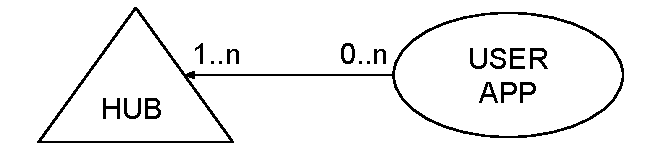
\includegraphics[width=0.7\textwidth]{Figures/system_architecture}
\caption{Architecture of the system}
\label{architecture_system}
\end{figure}

\begin{figure}[h]
\centering
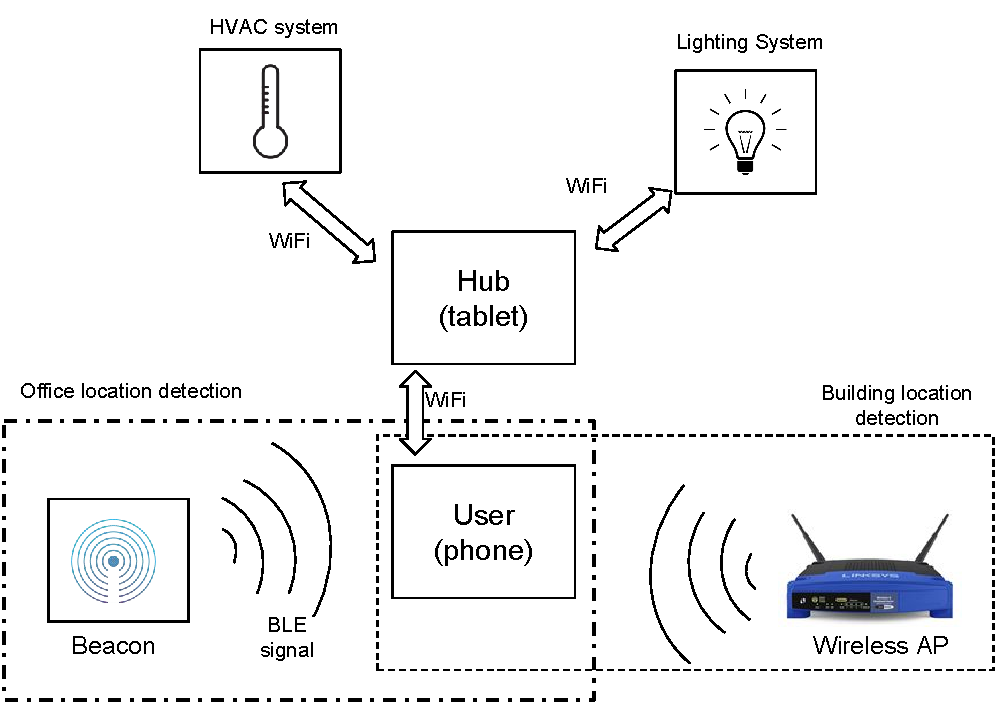
\includegraphics[width=0.9\textwidth]{Figures/harware_arch}
\caption{Overview architecture of the system}
\label{software1}
\end{figure}


\subsection{User App}

The User app runs in the user's mobile device and offers remote control of the lighting, \ac{HVAC} and security systems provided by the Hub. Besides improving user comfort by allowing remote access to the Hub, the user app also helps the Hub with user detection, allowing the system to know when an authorized user is inside the building or room.



\subsection{Hub App}

The Hub app is responsible for controlling the \ac{HVAC} and lighting systems in the office, enforcing energy saving policies, improving occupant comfort and providing security monitoring when the user is away from the office.

The main visual features of the Hub application are: a simple \ac{UI} to control the lights and heating/cooling system, an \ac{IFTT} automation system that allows the user to create personalize trigger/actions rules. In the background it also provides motion detection and video recording for occasions when the user left the room but movement is detected.


\section{Hardware Architecture}\label{architecture3} 

To achieve building automation, our solutions requires a tablet to act as a central control unit, a beacon device used for user detection inside the room and two other devices capable of interacting with the lighting and \ac{HVAC} systems.

The tablet is where the Hub app is executed. It provides the sensors, the connectivity, the storage as well as a camera, microphone, speaker and a touch screen. 

The beacon is used for user detection, this will be explained latter in Section~\ref{architecture4}.

To control the lighting and \ac{HVAC} systems we require devices capable of interacting with existing systems that offer a way to remotely control these existing systems. These devices can be for example microcontrollers. A microcontroller allows the digital world to interact with the real world through the use of actuators that convert electric signal into mechanical actions. The microcontroller is connected to the actuators (relay) and is able to switch on/off the lights as well as controlling the HVAC. This component is needed because typically, lighting and HVAC systems do not have any type of connectivity other than the electric wires. 


If the room had wireless devices that communicate with technologies such as ZigBee or Z-Wave installed, then the microcontroller could be connected to a radio module able to communicate with those wireless technologies such as a xbee module.


Figure \ref{harware_arch}, represents a Hub, its components and the main communication protocols used.

 

\subsection{Communication Protocols}

The system requires that the Hub and User App, are able to communicate with each other. They will use Wi-Fi to communicate data at high data rate. The Hub can also use \ac{BLE} to get additional sensor data from external sensors. Likewise the User App can use \ac{BLE} to determine if it is close to a beacon. The communication between the Android tablet and the microcontroller is done using an WiFi network. Finally the communication among the microcontroller and the actuators is done by using the General Purpose Input/Output (GPIO) pins.




\begin{figure}[h]
\centering
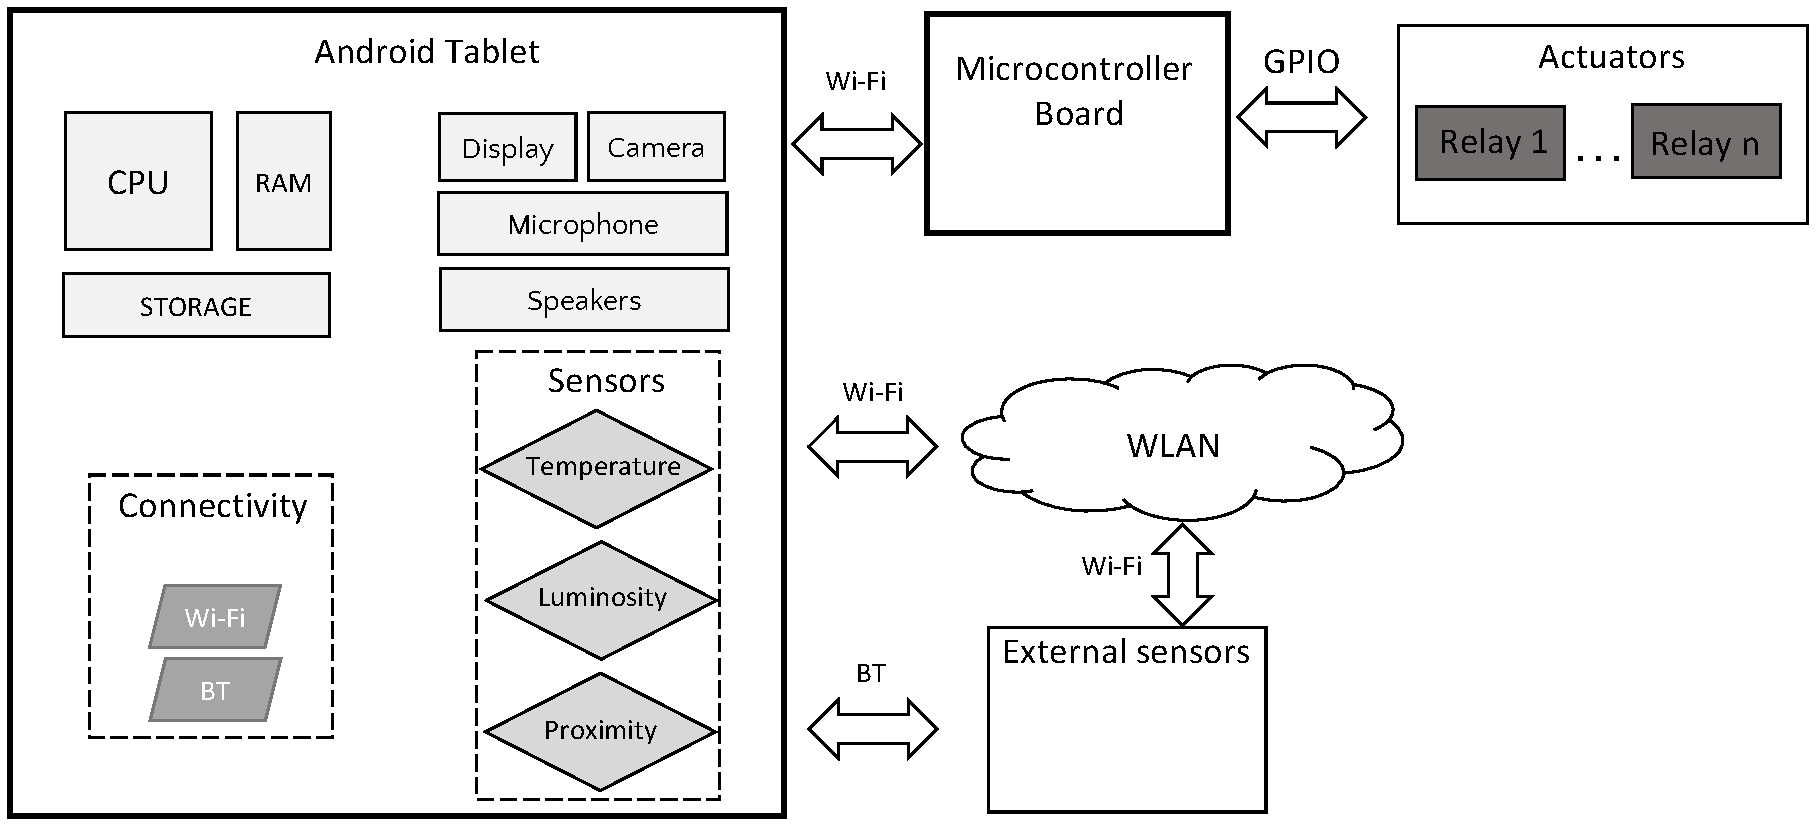
\includegraphics[width=0.9\textwidth]{Figures/arch_hardware}
\caption{Hardware architecture of the Hub}
\label{architecture_system}
\end{figure}


\section{Software Architecture}\label{architecture4} 

In this section we present the software architecture for the mobile apps and explain some of the core functionalities of our solution.

To achieve \textbf{building automation} we propose a \ac{IFTT} system. The user is able to create personalized chains of conditional statements, called "recipes", they are triggered based on events relevant to the office. With this system we could turn on the lights automatically when the user enters the room or shut them down when he leaves.

One of the goals of our solution is \textbf{user detection}, in order to accomplish this, we can leverage two different types of location systems: \ac{WiFi} and \ac{BLE} beacon location. The location detection is handled by the user app. We use the building's \ac{WiFi} network to determine if the user is inside the building by comparing the \ac{MAC address} of available \ac{AP}s to a set of known addresses. The other location system we can use is beacon location. There can be a beacon emitting \ac{BLE} signals and when this signal is detected, we know the user is near the beacon source (the office).

Regarding \textbf{office security}, we propose using the tablet's camera and analyzing the consecutive frames for changes. When no user is present in the room and a large enough number of pixels are different, we assume movement has occurred. We can then notify the user that someone is inside the room.


\subsection{Hub App Architecture}

This section presents the software of the HUB. This is comprised of several managers. Figure \ref{software2}, represents the architecture of the Hub App.

\subsubsection{User Interface}
This is the interface seen in the Hub screen, it will offer:

\begin{itemize}
  \item Manual control of the lighting and HVAC systems.
  \item User registration.
  \item Creation of automation rules.
  \item Real-time ambient sensors readings.
  \item Security settings, enable/disable security monitoring and notification email.
  \item General settings, activate voice control, allow sound.
   
\end{itemize}

\subsubsection{Communication Layer}

The Hub app implements a web server offering an \ac{REST} \ac{API} that the user app can use to interact with. 

The \ac{JSON} standard is used as the message format. This also means that in the future our system could communicate and be controlled by other devices using the \ac{API}.

\subsubsection{Event Manager}
The Event Manager offers publish/subscribe service. It allows other managers to register their interest in certain events and when those happen they are notified. There can exists several different types of events: temperature reading, motion detected, user detection, etc.

The Event Manager is also responsible for the automation logic by enforcing the \ac{IFTT} rules. The Automation Manager will check if the condition for the rule has been satisfied and trigger the action. 

Finally it also has a scheduler responsible for executing repetitive tasks at regular time intervals or at fixed moments.


\subsubsection{User Manager}
The User Manager handles user registration, authentication and detection. It tracks the whereabouts of the user inside the building, in association with the User app so that, it is notified when the user enters the building or office.


\subsubsection{Sensor Manager}
Sensor Manager allows access to the tablet's sensors as well as the external sensors. It abstracts external sensors into virtual sensors. It is responsible for a virtual motion detection sensor, by using the camera to detect changes that would indicate motion, as well as other data such as the opening and closing of the door.


\subsubsection{Lighting Manager}

This manager is responsible for managing the lighting system. It communicates with the lightning controller (microcontroller) and synchronizes the lights state with the \ac{UI} and vice versa.

\subsubsection{Temperature Manager}

The Temperature Manager periodically reads the room temperature and is able to communicate with the \ac{HVAC} controller (microcontroller) to turn on/off the system when required.


\begin{figure}[h]
\centering
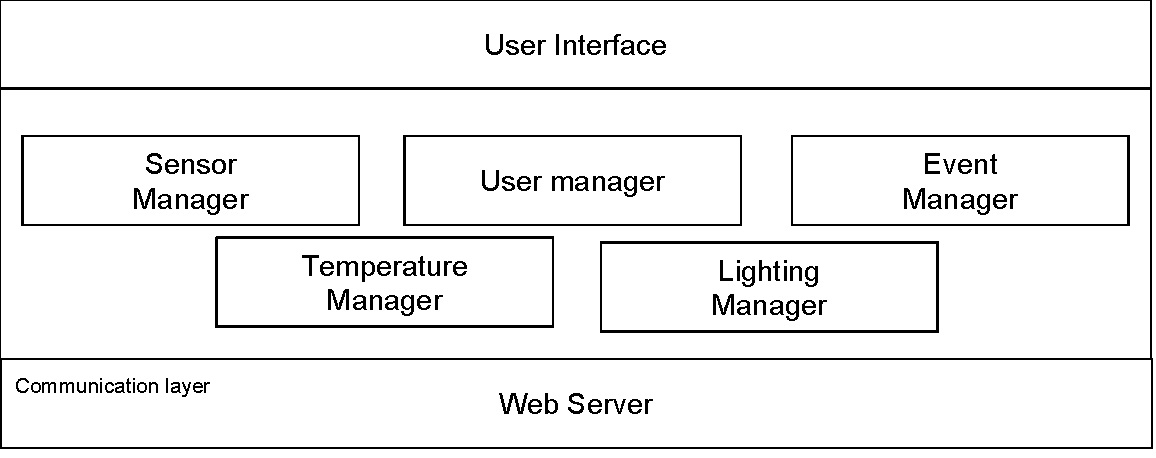
\includegraphics[width=0.9\textwidth]{Figures/software_hub}
\caption{Hub APP architecture }
\label{software2}
\end{figure}



\subsection{User App Architecture}
The User App is simpler than the Hub App, the app is divided in \ac{UI} screens. There are no managers like the Hub architecture, the business logic is handled by each screen separately. 


The main screens are the home, lighting, temperature, security and registration screens.

Since the user app can control several Hub apps, we require a simple registration process to add the user to the Hub. We propose showing a QR-Code in the Hub registration screen, this code possesses the \ac{IP } address for the Hub and a temporary token used for registration. The user app can use the phone camera to scan the QR-Code and automatically register the user in the Hub. Then a virtual representation of the Hub is shown in the home screen.

For user detection to work when the app is not being used, we need some kind of background service to monitor the \ac{WiFi} and beacons nearby the phone. The interval between scans will be further studied in order to provide adequate time between scans and be conservative regarding the user's mobile device battery.


